A simple combination is performed of the measurements from the ATLAS and CMS collaborations described in Sections~\ref{sec:HH_ATLAS} and \ref{sec:HH_CMS}.
The channels are treated as uncorrelated, in particular because the systematic uncertainties that we could expect to be correlated between the experiments, suche as the theory uncertainties and the luminosity uncertainty have little impact on the individual results.
The significance are added in quadrature and the negative-log-likelihood are simply added together. A summary of the different expected significances, as well as the combination, are shown in Table~\ref{tab:comb_significance}. The minimum minimum negative-log-likelihood are shown in Figure~\ref{fig:comb_HH}.

The trilinear coupling modifier is measured to be:
%\begin{equation}
\[
\begin{split}
1^{+XX}_{-XX} [^{+XX}_{-XX} (stat) ^{+XX}_{-XX} (syst)] \text{ at 68\% CL} \\
1^{+XX}_{-XX} [^{+XX}_{-XX} (stat) ^{+XX}_{-XX} (syst)] \text{ at 95\% CL}
\end{split}
%\end{equation}
\]

Assuming the SM HH signal the expected exclusion significance for the \kl\ = 0 hypothesis, i.e. no Higgs self-coupling, is XX and XX standard deviations with and without systematic uncertainties respectively.




\begin{table}[htb!]
\begin{center}
\begin{tabular}{lcccc} \toprule
 & \multicolumn{2}{c}{\textbf{Statistical-only}} & \multicolumn{2}{c}{\textbf{All Systematics}}\\
 & ATLAS & CMS & ATLAS & CMS \\
\hline
$HH \rightarrow b\bar{b}b\bar{b}$ & XX & XX & XX & XX \\
$HH \rightarrow b\bar{b}\tau\tau$ & XX & XX & XX & XX \\
$HH \rightarrow b\bar{b}\gamma\gamma$ & XX & XX & XX & XX \\
$HH \rightarrow b\bar{b}ll\nu\nu$ & - & XX & - & XX \\
$HH \rightarrow b\bar{b}ZZ(4l)$ & - & XX & - & XX \\
combined &  XX & XX & XX & XX \\
%$HH \rightarrow b\bar{b}b\bar{b}$ & 1.39 & XX & 0.61 & XX \\
%$HH \rightarrow b\bar{b}\tau\tau$ & 2.46 & XX & 2.13 & XX \\
%$HH \rightarrow b\bar{b}\gamma\gamma$ & 2.10 & XX & 2.03 & XX \\
%$HH \rightarrow b\bar{b}ll\nu\nu$ & - & XX & - & XX \\
%$HH \rightarrow b\bar{b}ZZ(4l)$ & - & XX & - & XX \\
%combined &  3.54 & XX & 3.02 & XX \\
\hline
 &  \multicolumn{2}{c}{Combined} & \multicolumn{2}{c}{Combined}\\
 &  \multicolumn{2}{c}{XX} & \multicolumn{2}{c}{XX}\\
\bottomrule
\end{tabular}
\end{center}
\caption{Significance in standard deviation of the individual channels as well as their combination.}
\label{tab:comb_significance}
\end{table}



\begin{figure}[!htb]
\centering 
\subfloat[]{\label{fig:comb_HH_a}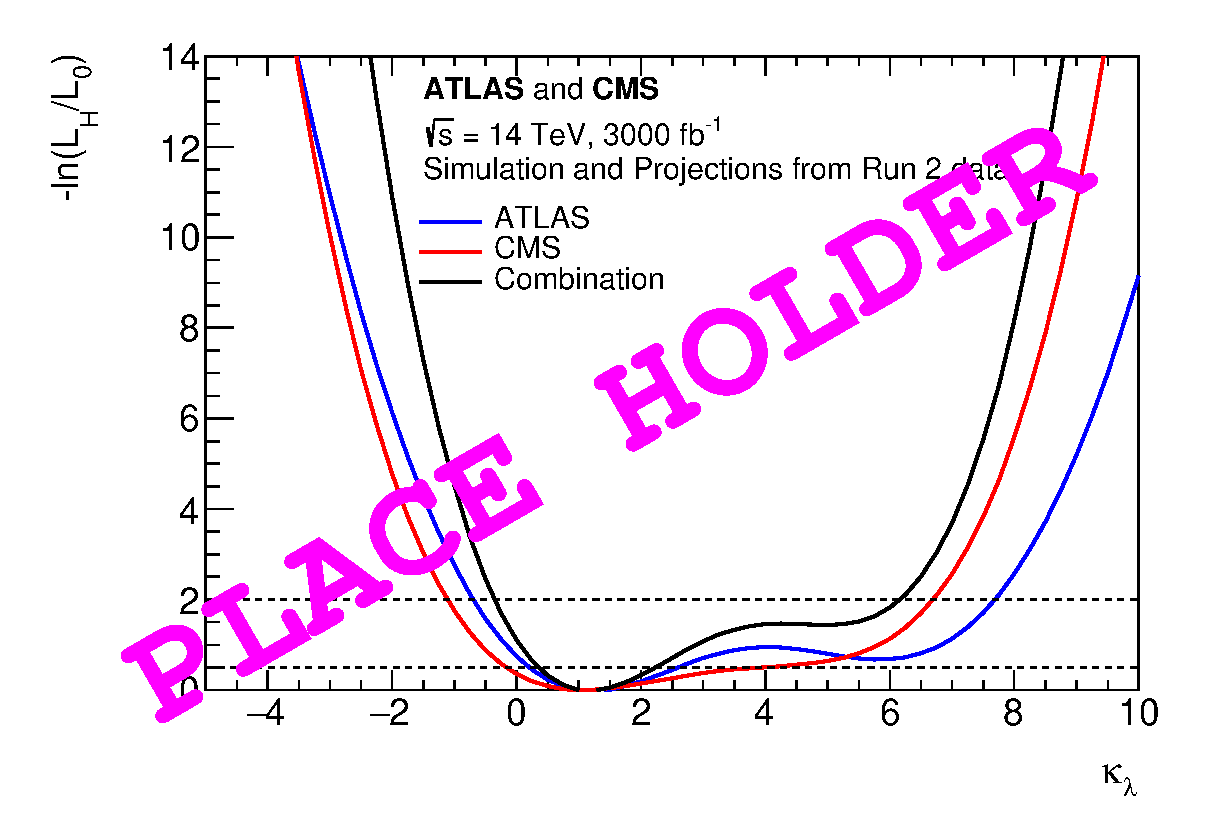
\includegraphics[width=0.5\textwidth]{\main/section3/plots/LHcombined_placeholder}} 
\subfloat[]{\label{fig:comb_HH_b}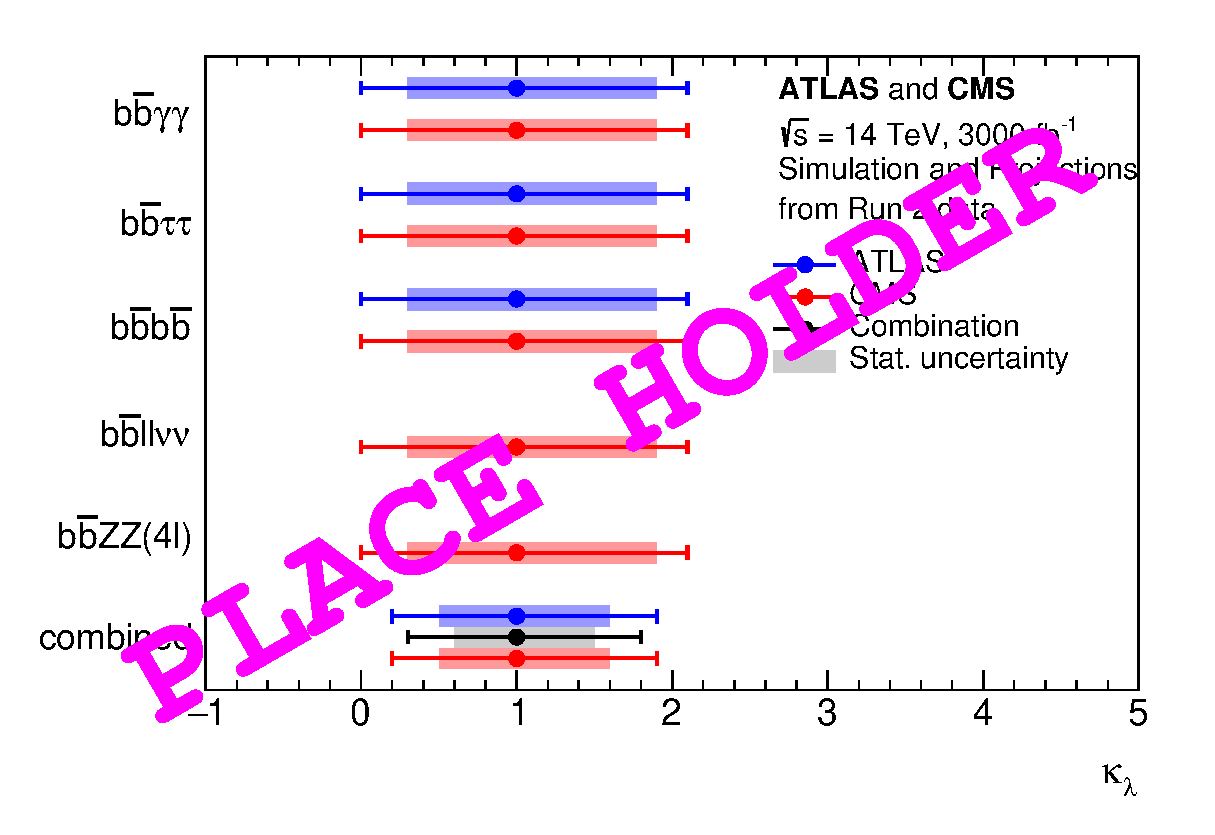
\includegraphics[width=0.5\textwidth]{\main/section3/plots/UncertaintyKappaLambda_placeholder}} 
\caption{(a) \textcolor{red}{PLACEHOLDER, DUMMY NUMBERS} Minimum negative-log-likelihood as a function of \kl, calculated by performing a conditional signal+backgrond fit to the background and SM signal. The blue and red lines correspond to the ATLAS and CMS results and the black line to the combined result. The dashed lines at $-ln(L_{H}/L_{0})$ = 0.5 and 2 indicates the values corresponding to a 1~$\sigma$ and 2~$\sigma$ confidence interval respectively (assuming an asymptotic $\chi^{2}$ distribution of the test statistics). (b) \textcolor{red}{PLACEHOLDER, DUMMY NUMBERS} Expected measured values of \kl\ for the differents channels for the ATLAS in blue and the CMS experiment in red, as well as the combined measurement. The black error bars show the total uncertainty on each measurement while the boxes correspond to the statistical uncertainties.} 
\label{fig:comb_HH} 
\end{figure}
